\chapter{Testing Framework Implementation}
\label{chap:implementation}

This chapter describes the modelisation of the problem, the block building
strategies that have been implemented in order to validate the correctness of
the proposed model, and the methodology that has been employed to test the
framework.

\section{Modelisation}
\subsection{Metrics}
\FloatBarrier
A way to rationally compare strategies is needed in order to discuss their
relative strengths and weaknesses. Three main characteristics will be used for
that:
\begin{itemize}
        \item latency;
        \item number of nodes;
        \item overhead.
\end{itemize}

\subsubsection{Latency}
The latency is the number of messages required to finalize a block and is a
measure of a blockchain's liveness. Latency should be as close to two so as to
reach finality as soon as possible \todo{explain why a latency of two is the
  minimum (and for n validators, it will be $2 \times
  safety\_threshold/validator\_weight$, assuming uniform weight distribution).
  Maybe more appropriate in Chapter 2:Finality though}
and the closer the latency is to the ideal
value, the more alive the system is as transactions take less time to be
confirmed.

\subsubsection{Number of nodes}
The number of nodes in the validator set and should be as high as possible to
guarantee decentralization and safety.

\subsubsection{Overhead}
The overhead is the number of messages that are sent over the network between
one step of the consensus and the next. It should be as low as possible to keep
the costs in bandwidth low.

\subsubsection{Example}

\begin{figure}[h]
	\centering
	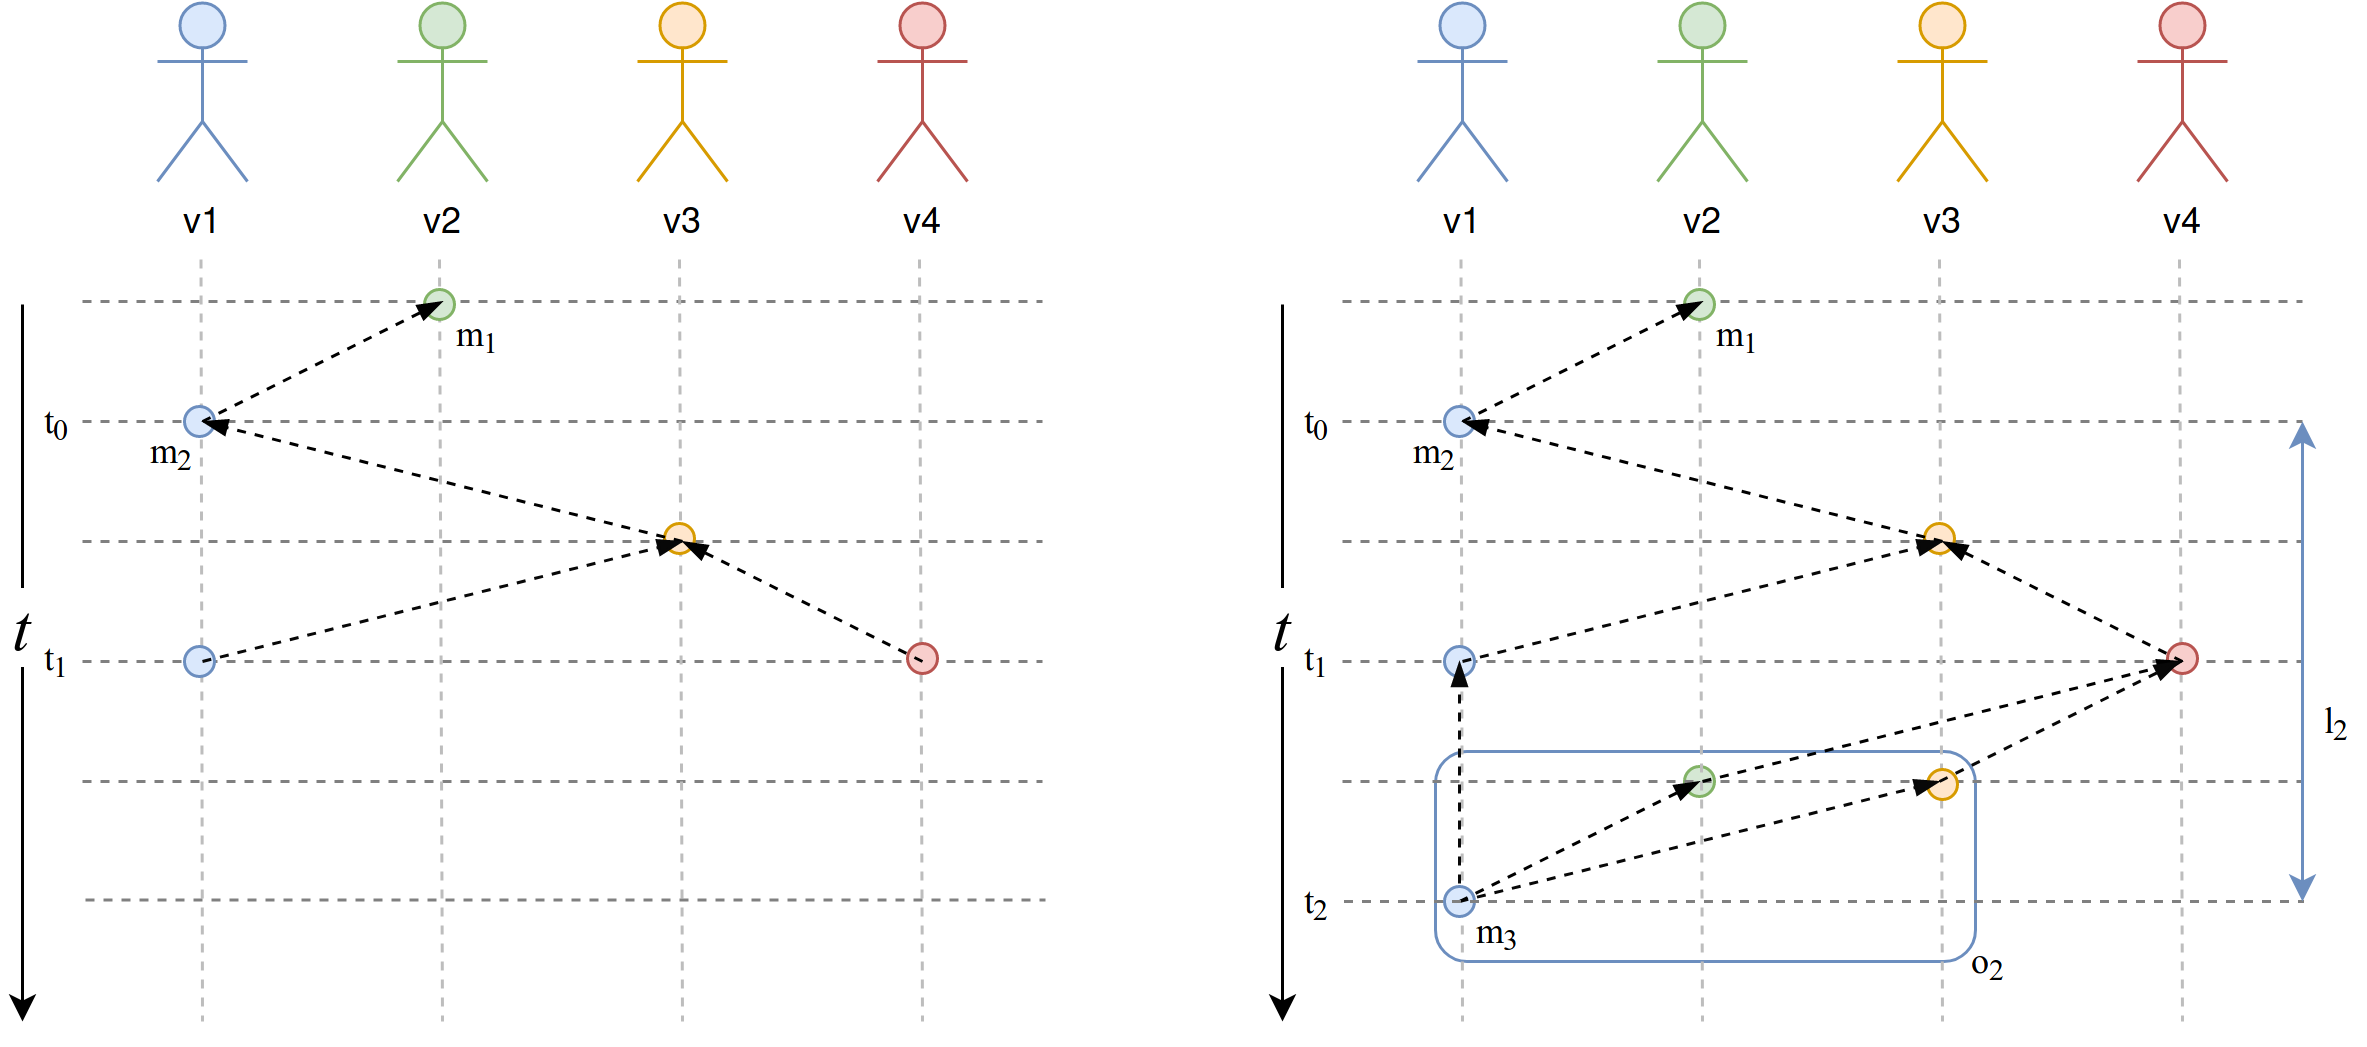
\includegraphics[width=\columnwidth]{metrics-example}
  %\captionsetup{justification=centering}
    \caption{Metrics computation example}
	\label{fig:metricsSchema}
\end{figure}

\fig{fig:metricsSchema} portrays how the metrics are computed: the left half of
the Figure is the initial states of the system at time \(t_1\) where message
\(m_1\) is finalized. The other half of the Figure is the same system at time
\(t_2\) when \(m_2\) is finalized. The latency of \(m_2\) is \(l_2\)
-represented by the difference in heights between \(m_3\) and \(m_2\)- which is
worth 4 in this case. The overhead is measured by counting the number of
messages that have been sent between \(t_1\) and \(t_2\), worth 3.

\FloatBarrier

\subsection{Tradeoff triangle/Trilemma}
In a standard consensus protocol, the three metrics form a trade-off triangle in
kind of a ``pick two'' fashion. \todo{not a pick two} \gls{cbc}-Casper has no
assumptions on timings, sources, contents, destinations of the messages that are
exchanged, and can therefore explore the whole trade-off space. This project
aims to find strategies that span the entirety of the triangle and
\todo{finish sentence what}

\subsection{Basic model}
\label{ssec:model}
The first strategy evaluation model that was chosen is:

\[1 = s_n \cdot \frac{1}{n} + s_l\cdot l + s_o\cdot o\]


This model binds each 3 variable \(n\) (number of nodes), \(l\) (latency) and
\(o\) (overhead) to their score \(s_{variable}\).
}


The higher the score \(s_x\) is, the more its related variable is dominant in
the strategy and therefore the closer to a corner of the triangle the strategy
is.  \(\frac{1}{n}\) is used because a large number of nodes is wanted.  The
basic model has linear dependencies between scores and variables and is probably
highly inaccurate but serves as a decent starting point to analyze the
simulation dataset.

\subsection{Model Evaluation}
After running the strategies in the simulation environment, metrics for \(n\),
\(l\) and \(o\) have been recorded. Then, for multiple runs, a linear regression
has been performed in order to find the scores \(s_x\).

\section{Strategies}
\label{sec:strategies}

The following strategies were proposed in order to visit known parts of the
trade-off triangle:
\begin{itemize}
        \item round-robin;
        \item double round-robin;
        \item triple round-robin;
        \item maximal overhead;
        \item arbitrary.
\end{itemize}
These strategies should allow one to visit the whole triangle and to discuss
their respective strength and weaknesses. The following sections describe the
strategies as well as their expected locations in the triangle.

\begin{figure}[h]
	\centering
	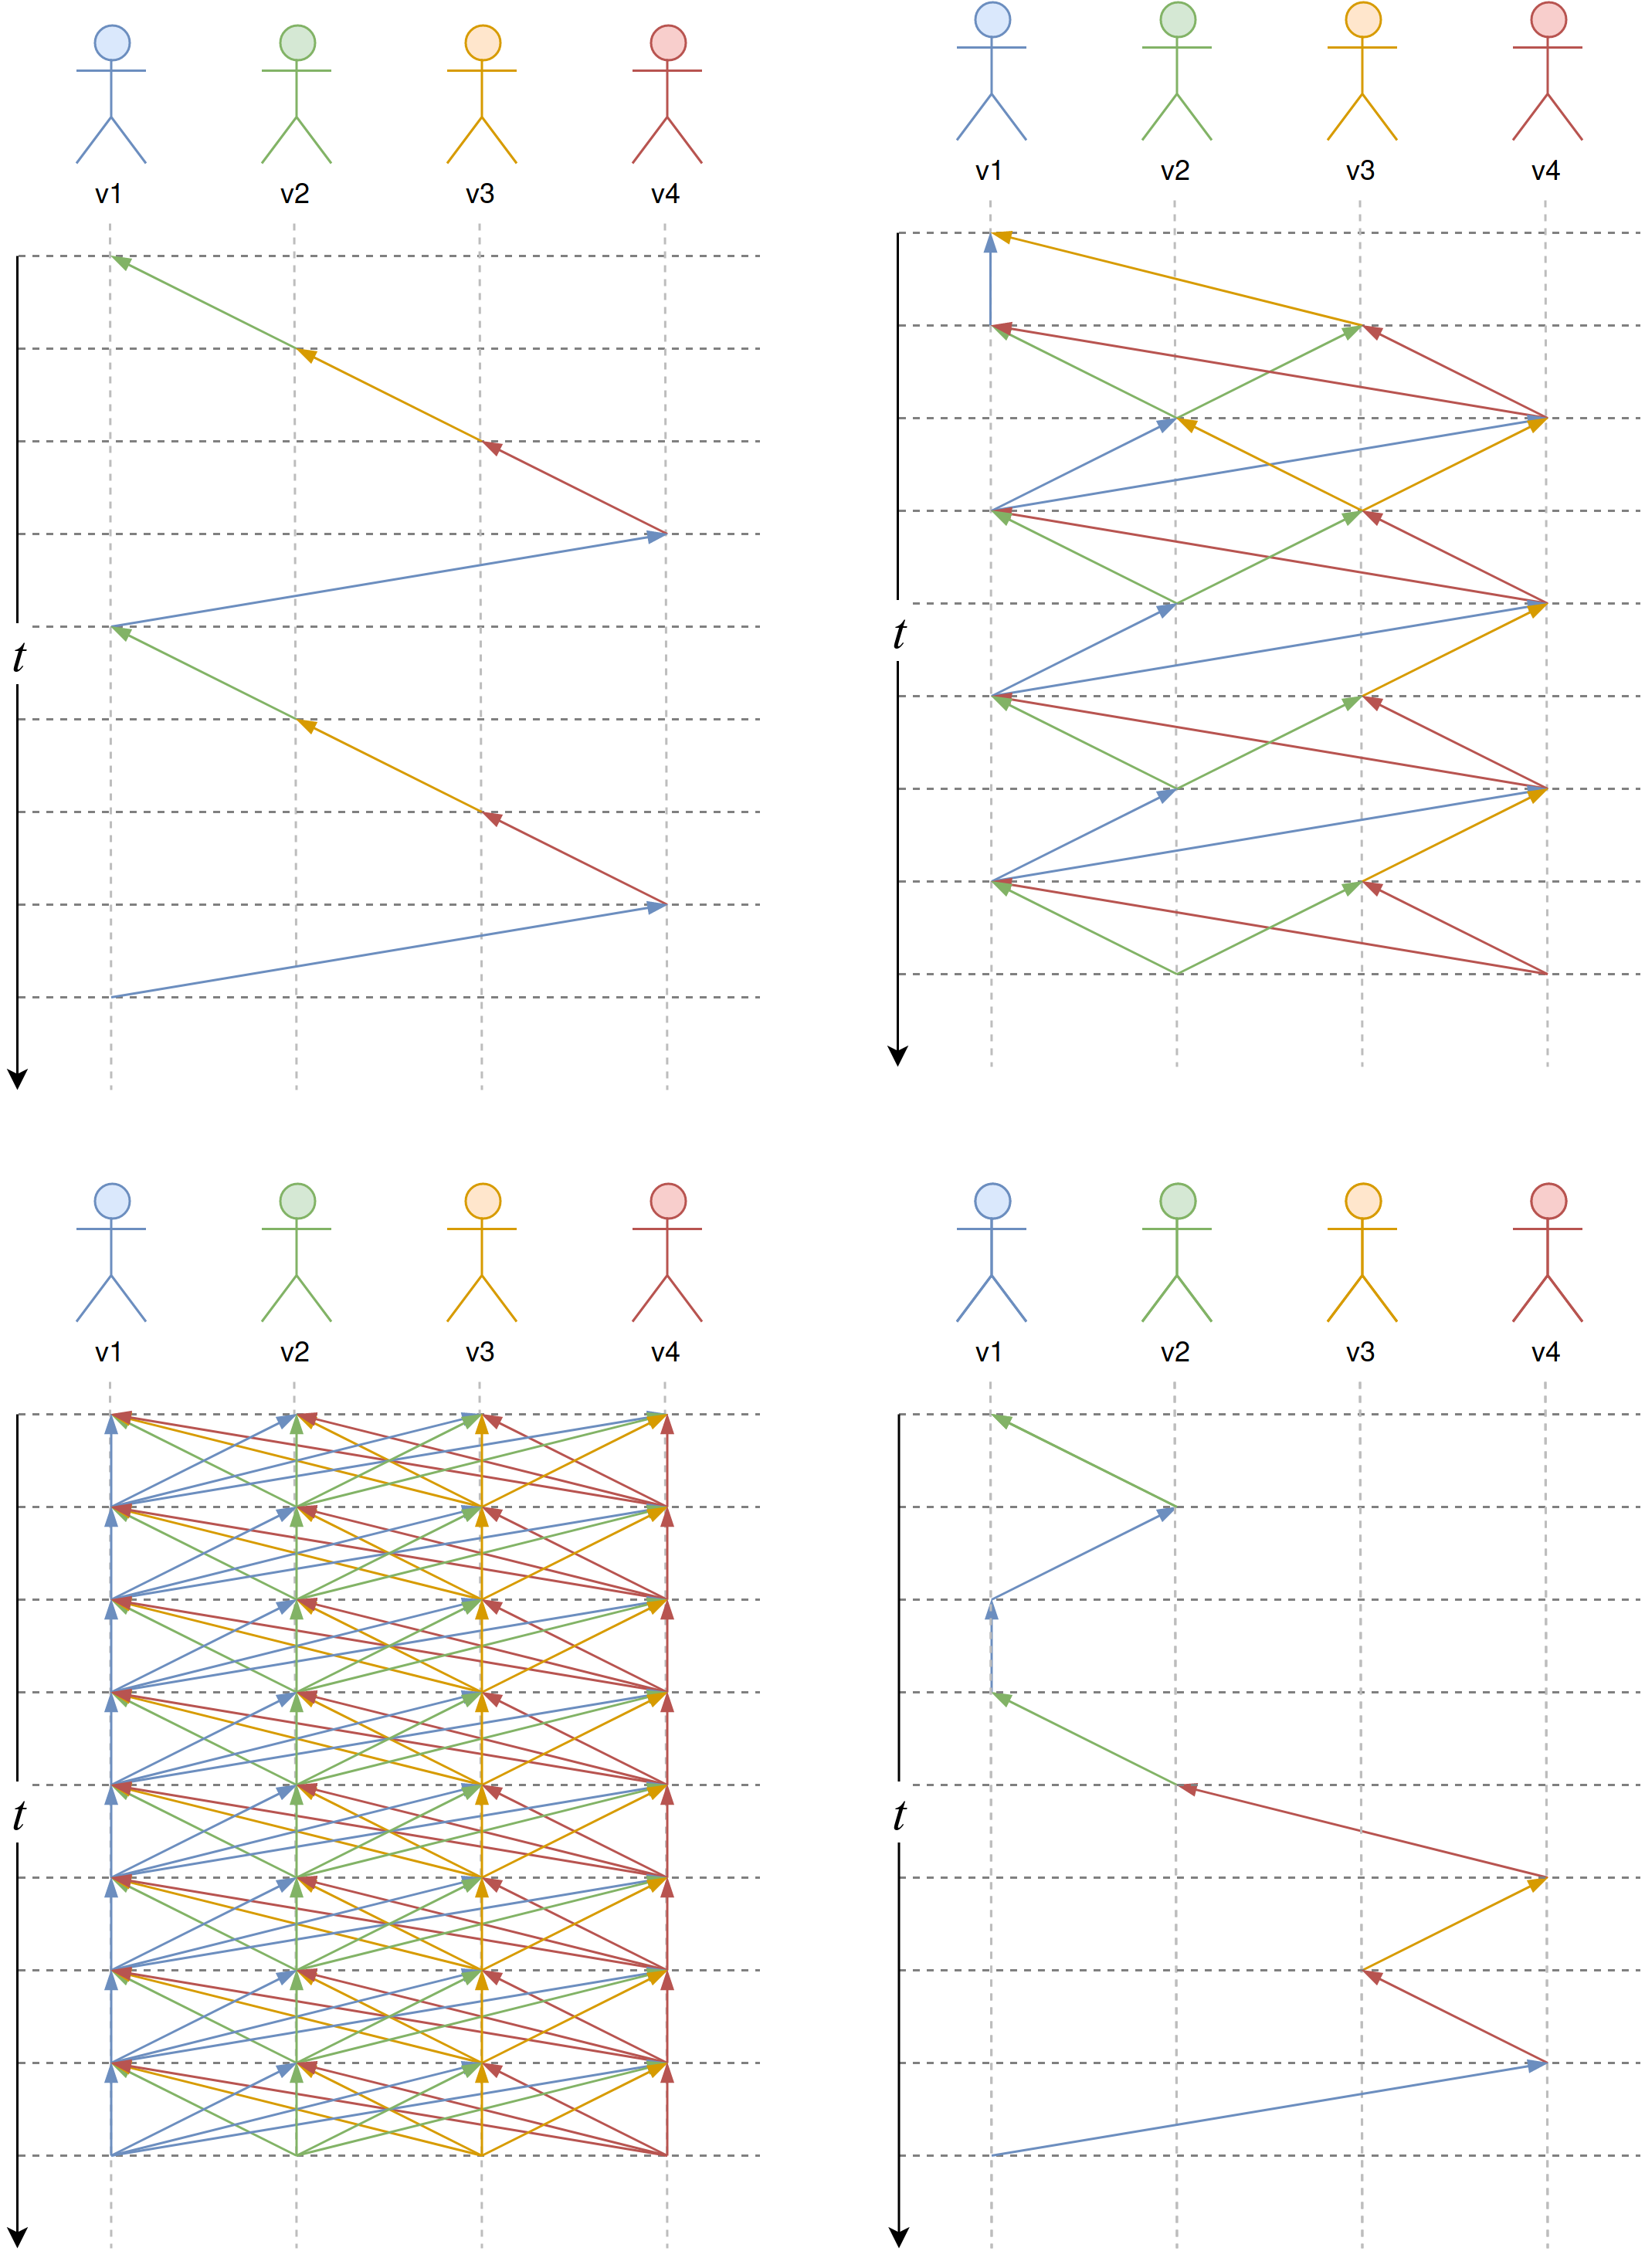
\includegraphics[width=0.8\columnwidth]{all_strats}
  %\captionsetup{justification=centering}
    \caption{Strategies examples with 4 validators. Top-left: Round-robin.
    Top-right: Double round-robin. Bottom-left: Maximal overhead. Bottom-right:
    Arbitrary. Arrows here show justifications for all messages.\todo{ref}}
	\label{fig:allStrats}
\end{figure}

\subsection{Round-robin}
Nodes send messages one after the other in a fixed order. The expected overhead
for this strategy should be the lowest of all the strategies as only one
message is sent at a time and each sent message should finalize a new block.
The latency, on the other hand, should be quite high because as seen in
\ssec{ssec:cbc} \(50\%\) of the validators have to acknowledge the messages to
finalize them. Since the round-robin has a fixed rotation order for the
message production, finalization happens only a rotation and a half later, where the
first rotation acknowledges the message's existence and the subsequent half rotation confirms acknowledgment.


\subsection{Double Round-robin}
In this setting, two nodes send messages at the same time, in a fixed order. If
the two nodes that send messages at the same step are as far as possible from each
other in the set of validators, the latency to finality is supposedly
half as much as the simple round-robin strategy, as the whole validator set
sends a message in half the number of steps. The overhead is however
doubled because two messages are sent at each step.
\todo{remove - before cbc and casper}

\subsection{Triple Round-robin}
This strategy is similar to the Double round-robin, except that three nodes send
a message at each step. It was decided to add this strategy at a later stage of
the project in order to have intermediate comparison points between the Double
round-robin and the Maximal overhead strategy. As for the Double round-robin
strategy, the latency should be divided by three compared to the simple
round-robin and the overhead should be three times higher.
Note that a \(N\)-parallelized round-robins could be implemented in order to change the
position in the trade-off triangle but it would lose meaning for a number of
nodes smaller than \(N\) so there is no quadruple (or bigger) round-robin
implementation.

\subsection{Maximal Overhead}
This strategy is the most expensive in terms of bandwidth; at each step, each
validator sends a message to all others. This example strategy should give a
baseline value for the maximum overhead that is reachable in the tradeoff
triangle. It also minimizes the latency as only two steps are needed in order to
finalize a block. This strategy is similar to the pBFT\cite{pBFT} protocol
because each node sends a message to every other one over two steps.

\subsection{Arbitrary}
The Arbitrary strategy is the simplest to think of: pick a sender at random.
Using fixed probability density functions, one node is arbitrarily selected at
each step to create a message. This strategy could be modified in the same way
the simple Round-robin has evolved into the Double and Triple round robin
strategies to show the evolution of the metrics with the number of messages sent
at each step.

\subsection{Bottom-up strategies}
\label{ssec:bottomUpStrats}
All the previous strategies except Arbitrary require an overarching view
(``top-down'' view) of the system and the nodes to be synchronized.
Bottom-up strategies are more likely to be implemented from a real-life point of
view. Each node has its own view of the messages and acts in its own interest
based on that view.
For example a node could keep track of the whole state of the finalization of
messages, and only publish a message itself when it facilitates the
finalization. That kind of strategy has not been implemented but the testing and
scoring framework allows one to easily add them.
Such strategies should implement incentives for the nodes not to spam the
network and include mechanisms to slash nodes not following some rules the
strategies dictate.

\section{Methodology}
Over the duration of this thesis, the \texttt{core-cbc} library included a
test framework called \texttt{proptest}. The testing framework that has been
implemented includes ways to simulate the behavior of the Casper protocol over
multiple nodes and thousands of blocks. At the time of
writing, the simulations do not include network latencies.

\subsection{\texttt{proptest}}
\label{ssec:proptest}

The \texttt{proptest} implementation is able to run blockchain simulations off
the following parameters:
\begin{itemize}
    \item Number of validators;
    \item Terminating condition;
    \item Sender strategy;
    \item Receiver strategy.
\end{itemize}

\subsubsection{Number of validators}
The number of nodes that can validate blocks.

\subsubsection{Terminating condition}
The terminating condition is a predicate that tells whether or not the simulation has
reached an end. In this case, the end of the simulation is reached when at least
one node finds a safety oracle for a blockchain that has a height of 4. This
height was chosen because it offered a balance between the computation speed and
the variance in output values. If the chosen value was smaller the generated
blockchains would all look alike and some side effects would have been observed
near the genesis block whereas a bigger value would imply more computation time.

\subsubsection{Sender strategy}
The sender strategy selects one or more nodes that will create new messages and
forward them to the rest of the network. All the basic strategies that have been
presented in \sect{sec:strategies} are implemented as Sender strategies.
New strategies (including bottom-up ones) can be easily implemented as well.

\subsubsection{Receiver strategy}
Receiver strategies select a set of validators that receive messages created by
Sender strategies. Three strategies have been implemented for now: 
\begin{itemize}
        \item All receivers;
        \item Half receivers;
        \item Some receivers.
\end{itemize}

The \textit{all receivers} strategy broadcasts messages to each other validator.
The \textit{some receivers} strategy sends a message to \(1\) or more validator,
using a uniform probability density function.  As of now, none of the
implemented strategies are a good modelisation of a typical Ethereum network and
this will be fixed at a later iteration.  Nonetheless, these strategies offer
two extreme points on the spectrum of the network topology: a fully connected
one without latency (\textit{all receivers}), and a random one (\textit{some
receivers}) and will be both taken into account to compare the sender
strategies.
The \textit{half receivers} strategy sends a message to half the validator set,
chosen at random which has been implemented at a later stage of the project
because the \textit{some receivers} strategy ended up modifying multiple
parameters at once rendering the analysis of the output too complex for the
proposed model and tools.

\subsection{Metrics measurements}
\label{ssec:metricsMeasurements}

Metrics are not computed as-is in the \texttt{proptest} implementation. Simpler
data are logged into \texttt{csv} files, and are processed by a \texttt{Python}
script. The recorded data are: 

\begin{itemize}
    \item the number of nodes;
    \item the identity of the current node;
    \item the height of the chain;
    \item the height of the highest finalized block;
    \item and the total number of messages that have been sent.
\end{itemize}

This two step processing enabled the generation of
data before having a precise definition of the metrics. It also permits to vary
the way metrics are recorded. For example, from the same log file, you could
extract metrics only when the last step of the consensus is reached, or have an
average of the metrics at each step of the consensus.
